\clearpage{}
\section{Explain the goals and principles of software testing. Describe the
different stages of a software testing process, from unit to installation.
Discuss the different types of faults. Define and compare white-box and
black-box testing.}


\subsection{Software testing}

The goal of software testing is to \textbf{discover faults} and not to
demonstrate correctness (a test is successful when a fault is
discovered). When a fault is discovered, we identify the fault (what
fault caused the failure) and correct it (making changes to remove the
fault).

(testing $\neq$ proving)

\subsection{Stages of a software testing process}

\begin{figure}[!ht]
    \centering
    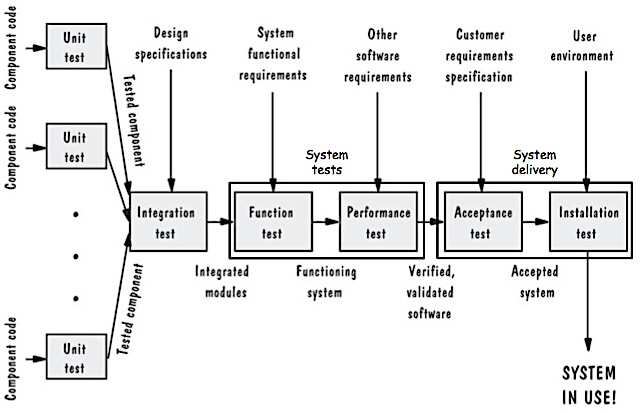
\includegraphics[width=0.8\linewidth]{stages_of_software_testing.png}
\end{figure}

\begin{description}
    \item[Unit test (aka.\ module test, component test)]
    Each program component.
    \item[Integration test]
    Assemble components together and check correct interaction.
    \item[Function test]
    The whole system.
    Check that the behaviour conforms to functional requirement specifications.
    \item[Performance test]
    The whole system.
    Check that the behaviour conforms to nonfunctional requirement specifications.
    \item[Acceptance test]
    The whole system.
    Test using the system with the customer.
    Check that the behaviour conforms to (customer) requirement documentation.
    \item[Installation test]
    The system in its operational environment.
    Check that the system performs properly in its environment.
\end{description}


\subsection{Types of faults}

\begin{description}
    \item[Algorithmic faults] the program logic produces a wrong computation
    \item[Computation and precision faults] a mathematical computation is wrong or the
    result does not have the required precision
    \item[Timing or coordination faults] incorrect event timing or
        coordination (real-time/concurrent systems)
    \item[Documentation faults] documentation doesn't match what program does
    \item[Throughput or performance faults] system's performance not acceptable
    \item[Capacity or boundary faults] System's performance not acceptable when activity
    increases
    \item[Hardware and system software faults] supplied hardware or system software does
    not work as specified
    \item[Standard and procedure faults] coding standards and procedures not respected
\end{description}

\subsection{White-box and black-box testing}

\begin{itemize}
    \item \textbf{Black box (or closed box)}: Content is unknown or ignored. 

        $\Rightarrow$ Test input/output behaviour (functional).

        \begin{itemize}
                \proitem{} Not constrained by the structure of the unit under test
                \consitem{} Impossible to know whether a test is complete
        \end{itemize}

    \item \textbf{White box (or clear box)}: Content is visible and observed. 

        $\Rightarrow$ Test internal operation (structural).

        \begin{itemize}
                \proitem{} Can check that program elements are tested
        \end{itemize}
\end{itemize}
